\documentclass[12pt]{article}

%Standard Stefanos Packages
\usepackage[utf8]{inputenc}
\usepackage{dirtytalk}
\usepackage{amsmath}
\usepackage{mathtools}  
\mathtoolsset{showonlyrefs} 
\usepackage{graphicx}
\usepackage{mdframed}
\usepackage{lipsum}
\usepackage{cancel}
\usepackage{systeme}
\usepackage{pgfplots}
\usepackage{textcomp}
\usepackage{geometry}
\usetikzlibrary{arrows}
\geometry{a4paper}
\graphicspath{ {./res/} }
\usepackage{float}
\restylefloat{table}
\newcommand{\comment}[1]{%
	\text{\phantom{(#1)}} \tag{#1}
}
\usepackage{subcaption}
\usepackage{graphicx}
\title{\line(1,0){450}\\ CS3DS19 - Data Science Algorithms and Tools \\ \large{Major Coursework }  \\\line(1,0){450} \\2021/2022}
\usepackage{pgfplots}
\author{Student ID: 27020363}
\newmdtheoremenv{note}{Note}
\pgfplotsset{compat=1.17}

%Extra Packages
\usepackage{tikz}
\usetikzlibrary{automata,positioning}

\usepackage{listings}
\usepackage{xcolor}

\definecolor{dkgreen}{rgb}{0,0.6,0}
\definecolor{gray}{rgb}{0.5,0.5,0.5}
\definecolor{mauve}{rgb}{0.58,0,0.82}

\usepackage{mathptmx}
\usepackage{setspace}
\setstretch{1.15}

\lstdefinestyle{myScalastyle}{
	frame=tb,
	language=scala,
	aboveskip=3mm,
	belowskip=3mm,
	showstringspaces=false,
	columns=flexible,
	basicstyle={\small\ttfamily},
	numbers=none,
	numberstyle=\tiny\color{gray},
	keywordstyle=\color{blue},
	commentstyle=\color{dkgreen},
	stringstyle=\color{mauve},
	frame=single,
	breaklines=true,
	breakatwhitespace=true,
	tabsize=3,
}
\begin{document}
	\maketitle
	\pagebreak
	
	\section{Task 1}
		
		In this Section, the  main parts of the workflow will be explained.
		\begin{center}
			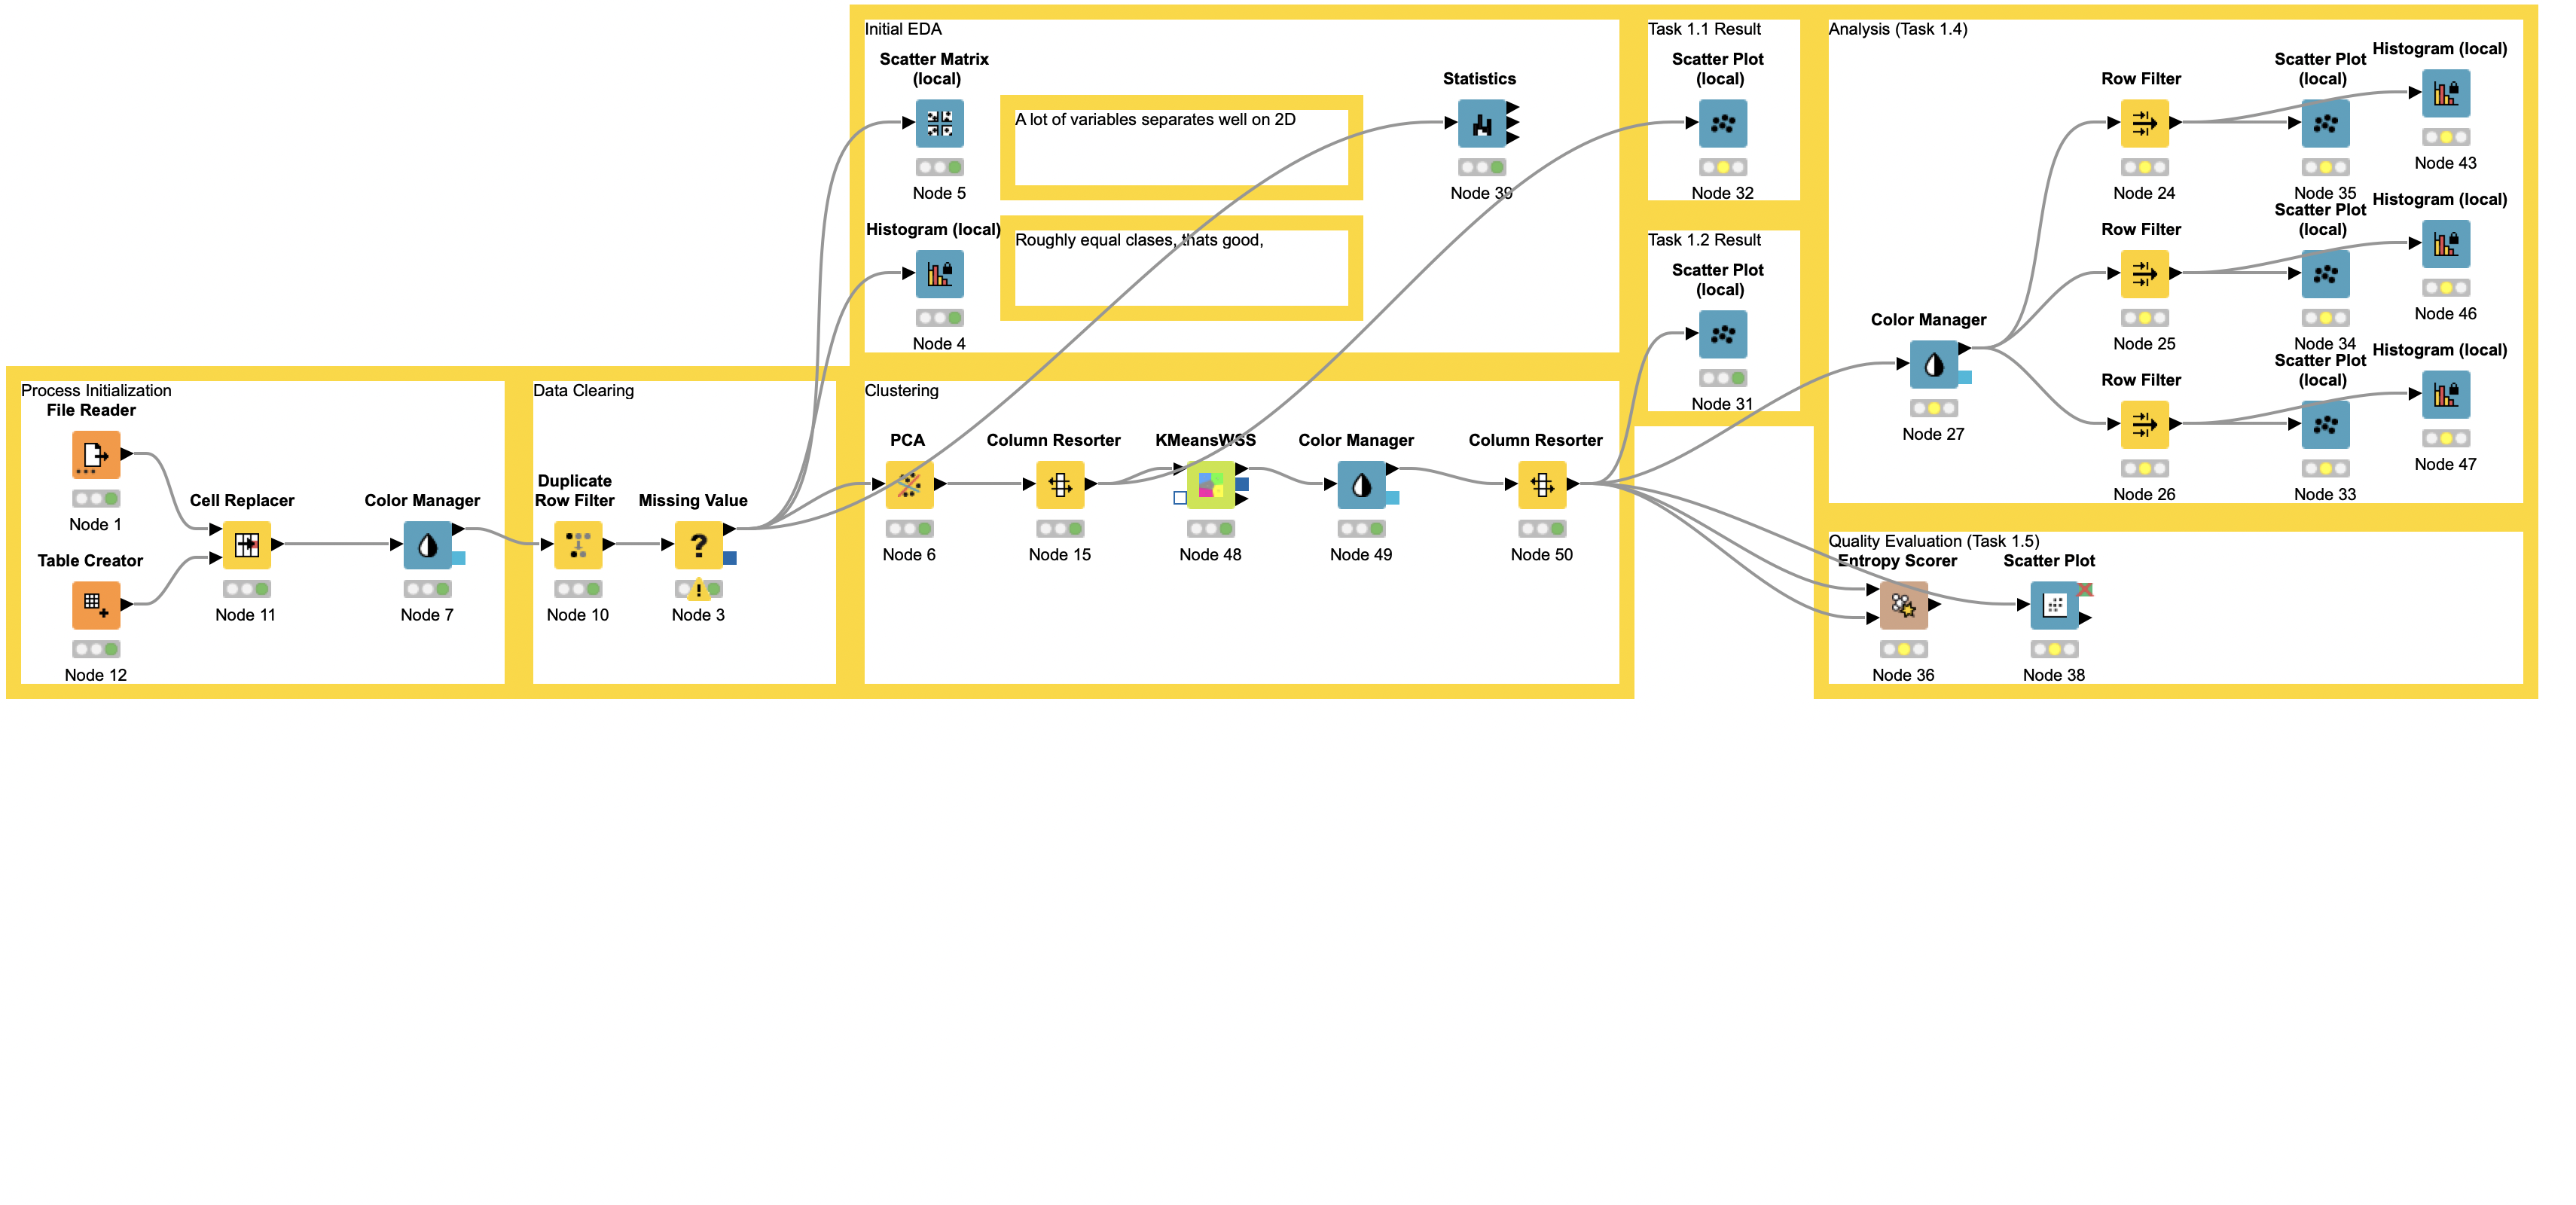
\includegraphics[scale=0.26]{res/workflow}
		\end{center}
		The workflow is splitted into 7 Stages. Those are
		\begin{itemize}
			\item Process Initialization : Read files, and transform the type of the class into string(was number). Finally we assign the initial colours for the subsequent plots, based on the classes field given by the dataset
			\item Data Clearing : Standard data clearing techniques, Drop duplicate data and missing values(by dropping all the rows involving missing data).
			\item Initial EDA : Some useful statistics that i used to get myself familliar with the data and their properties
			\item Clustering : PCA and KMeans Nodes(Futher Explaned below)
			\item Analysis : Evaluation of error, Classes distribution per cluster and histograms
			\item Quality Evaluation : Entropy scorer(Entropy/purity)
		\end{itemize}
	
	\section*{Task 1.1 : plot1}
	
	 	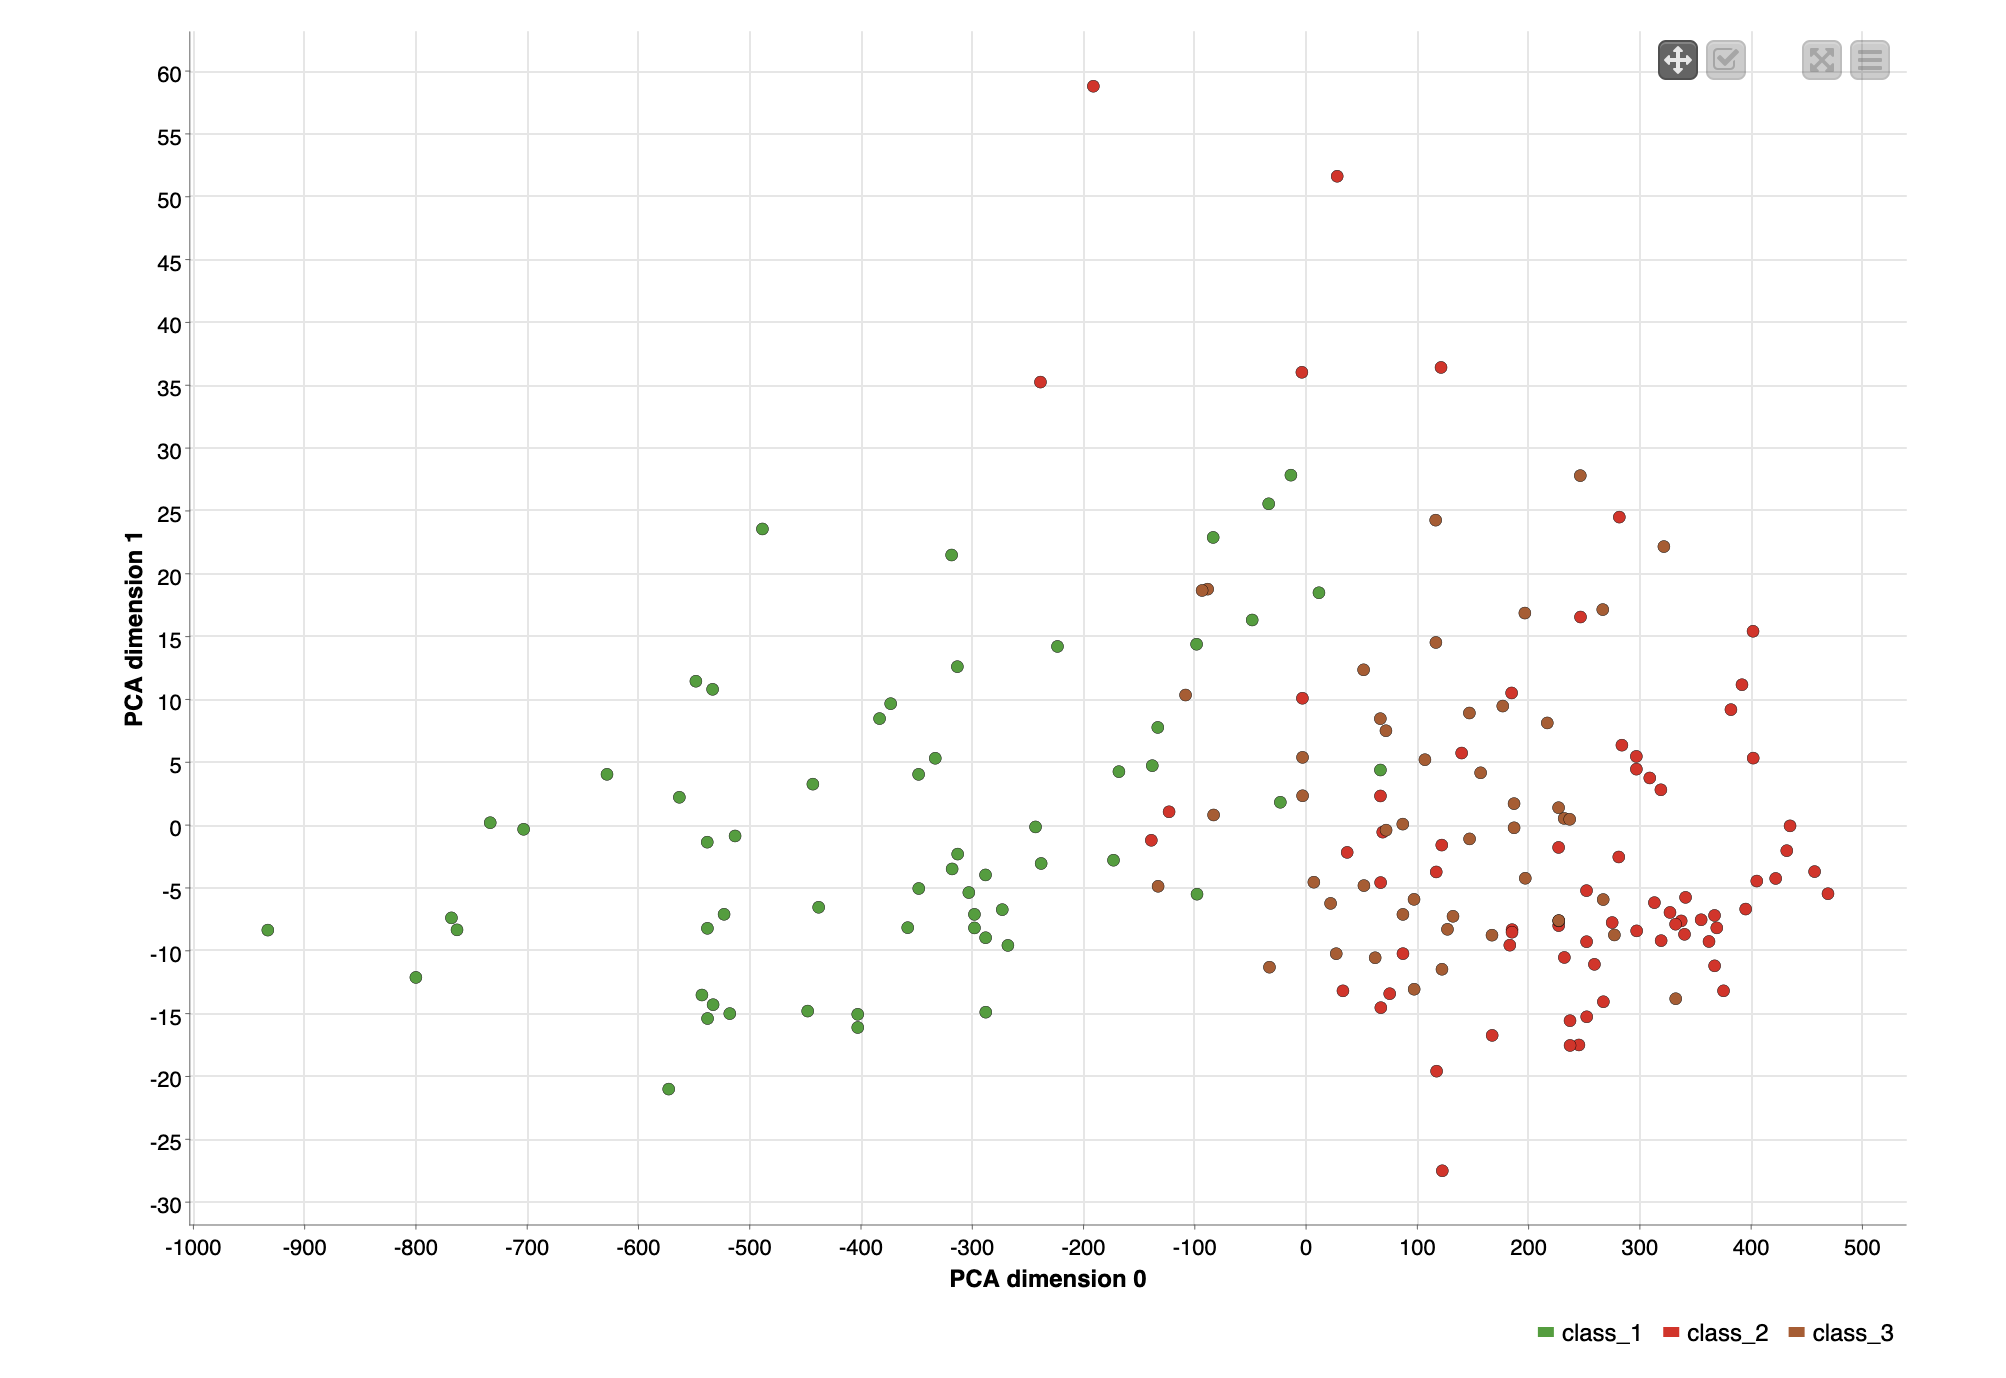
\includegraphics[scale=0.36]{res/plot1.1}
	 
	 \section*{Task 1.2 : plot2}
	 
	 	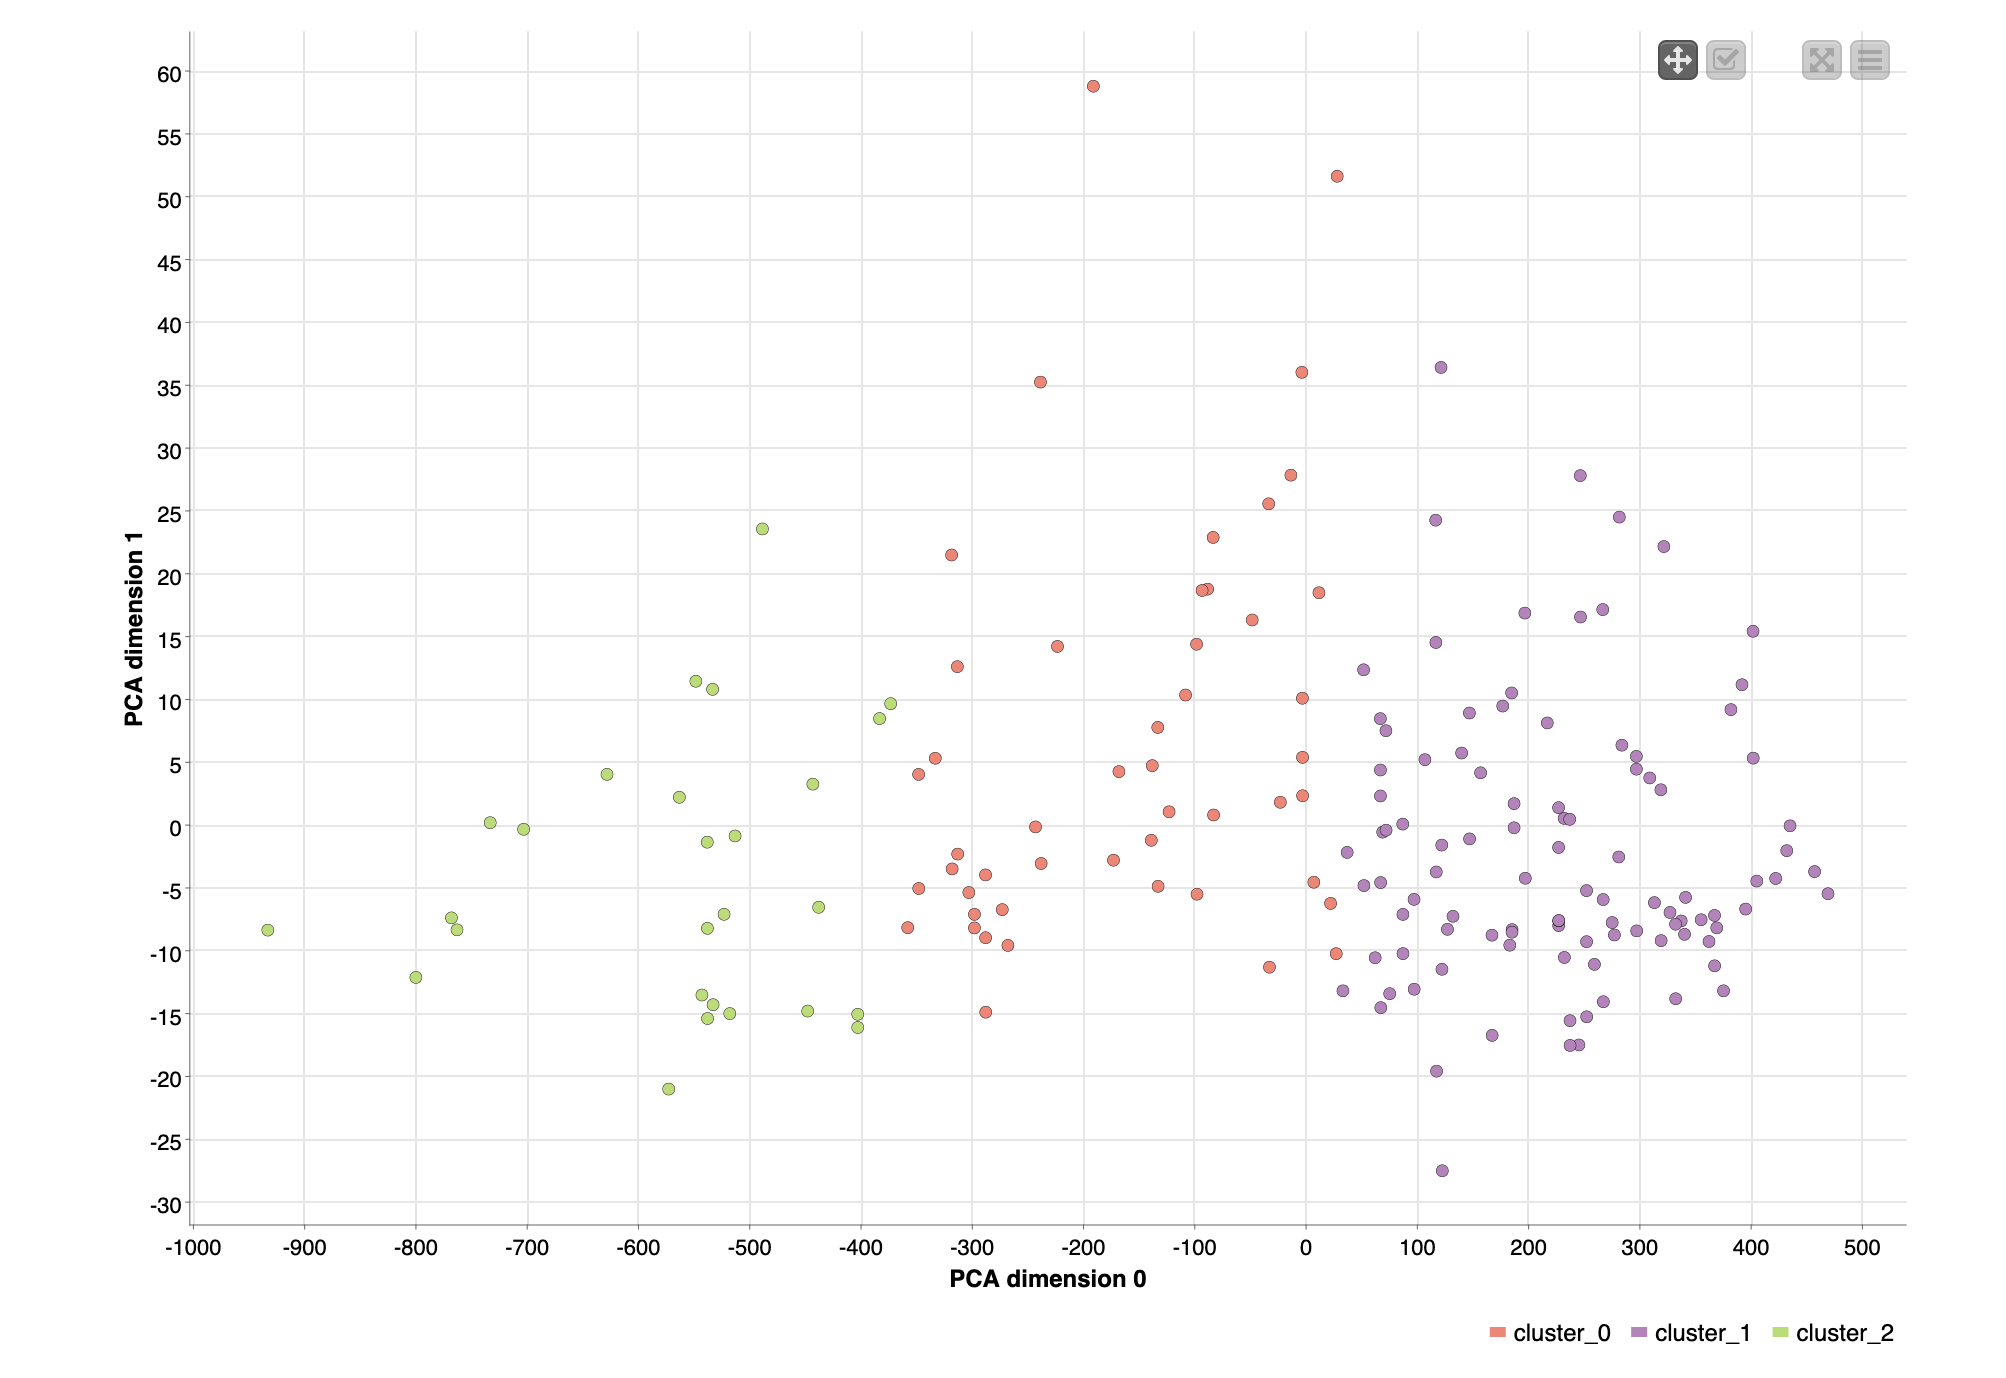
\includegraphics[scale=0.36]{res/plot1.2}
	 
	 \section*{Task 1.3 : compare, discuss and explain the differences between plot1 and plot2}
		The main point of interest in the figures above, is the fact that, the clustering algorithm(K-Means, k=3) failed to appropriately partition the data, and recognise the classes provided by the dataset. We can see that there are multiple errors(Detailed analysis per-class on Task 1.4). This phenomenon can be explained due to the absence of the standardization process, something that will be explained in the next Task. The exact scale of the problem cannot be appropriately assessed with only those two plots though, we will need to examine the distribution of the classes in each cluster, something that will be done on the next task(Task 1.4)
	
	 \section*{Task 1.4 : plot3a,plot3b,plot3c}
		The 3 requested plots are shown below
		 \begin{figure}[H]
		 	\centering
		 	\begin{subfigure}{0.4\textwidth}
		 		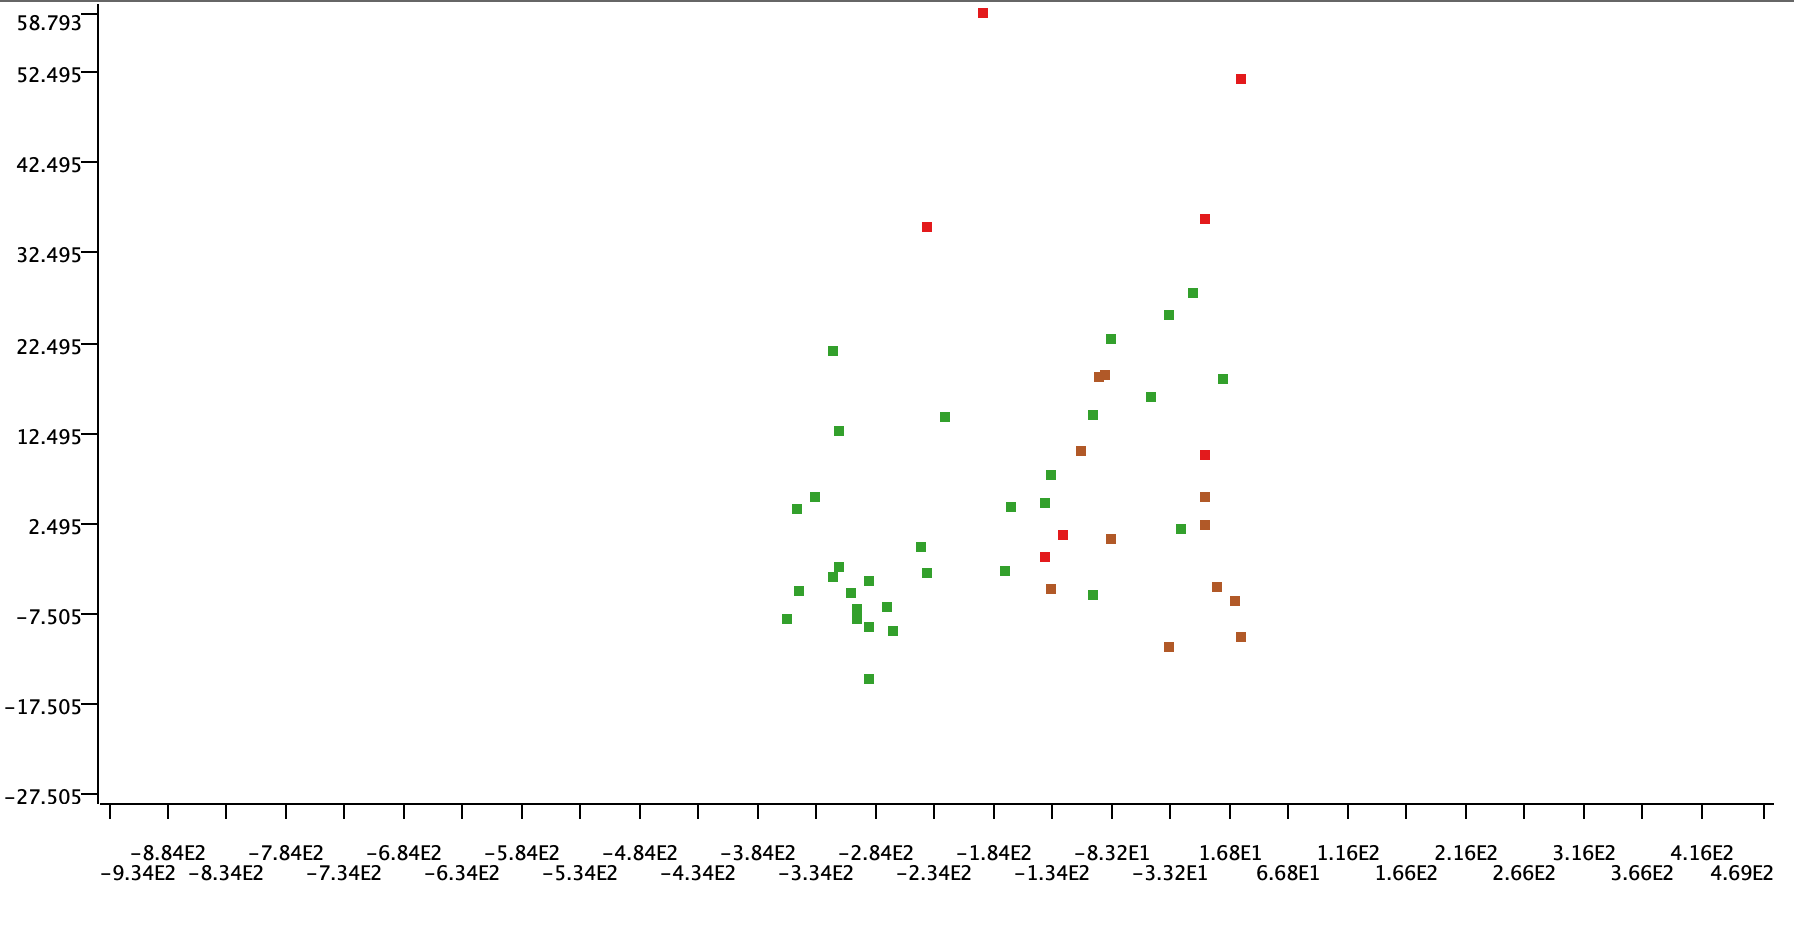
\includegraphics[width=\textwidth]{res/plot3a}
		 		\caption{plot3a}
		 		\label{fig:first}
		 	\end{subfigure}
		 	\hfill
		 	\begin{subfigure}{0.4\textwidth}
		 		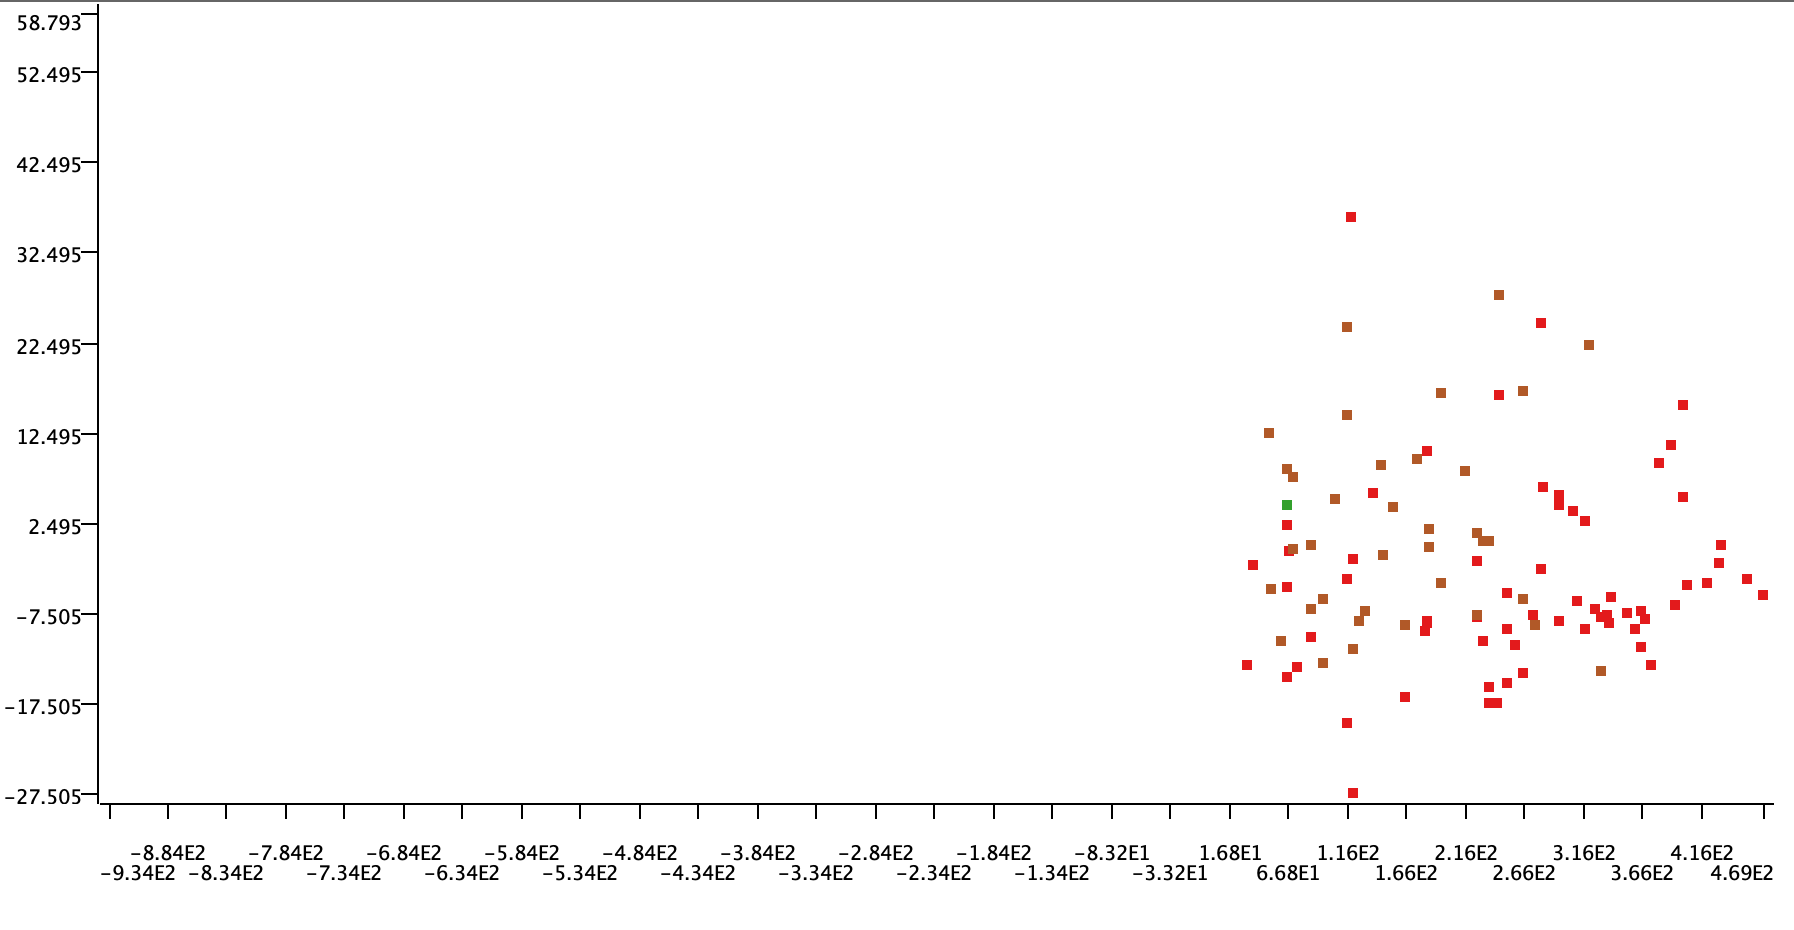
\includegraphics[width=\textwidth]{res/plot3b}
		 		\caption{plot3b}
		 		\label{fig:second}
		 	\end{subfigure}
		 	\hfill
		 	\begin{subfigure}{0.4\textwidth}
		 		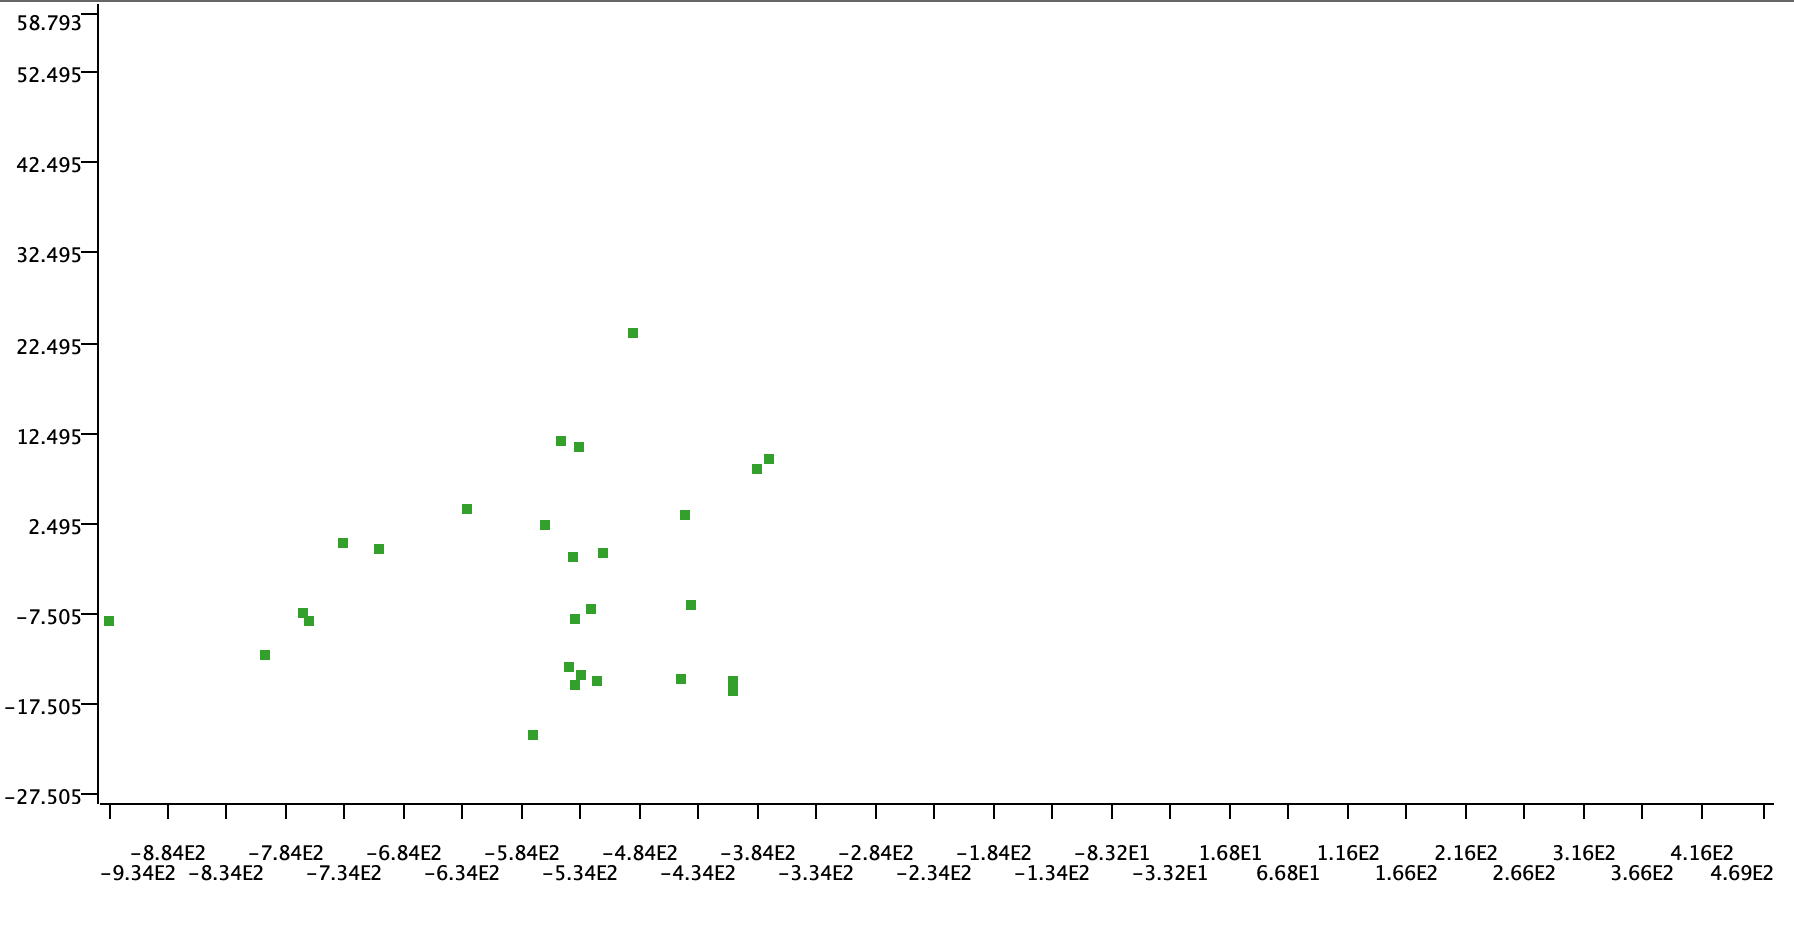
\includegraphics[width=\textwidth]{res/plot3c}
		 		\caption{plot3c}
		 		\label{fig:third}
		 	\end{subfigure}
		 	
		 	\label{fig:figures}
		 \end{figure}
		Here, we can see clearly each cluster and the classes of each datapoint that fails under those clusters. With use of histograms, we can learn the distribution of of classes in each cluster. Under ideal conditions(a good clustering), each cluster will contain the majority of the datapoints for some class, with a few missed points, unfortunately, this is not the case
		\begin{figure}[H]
			\centering
			\begin{subfigure}{0.4\textwidth}
				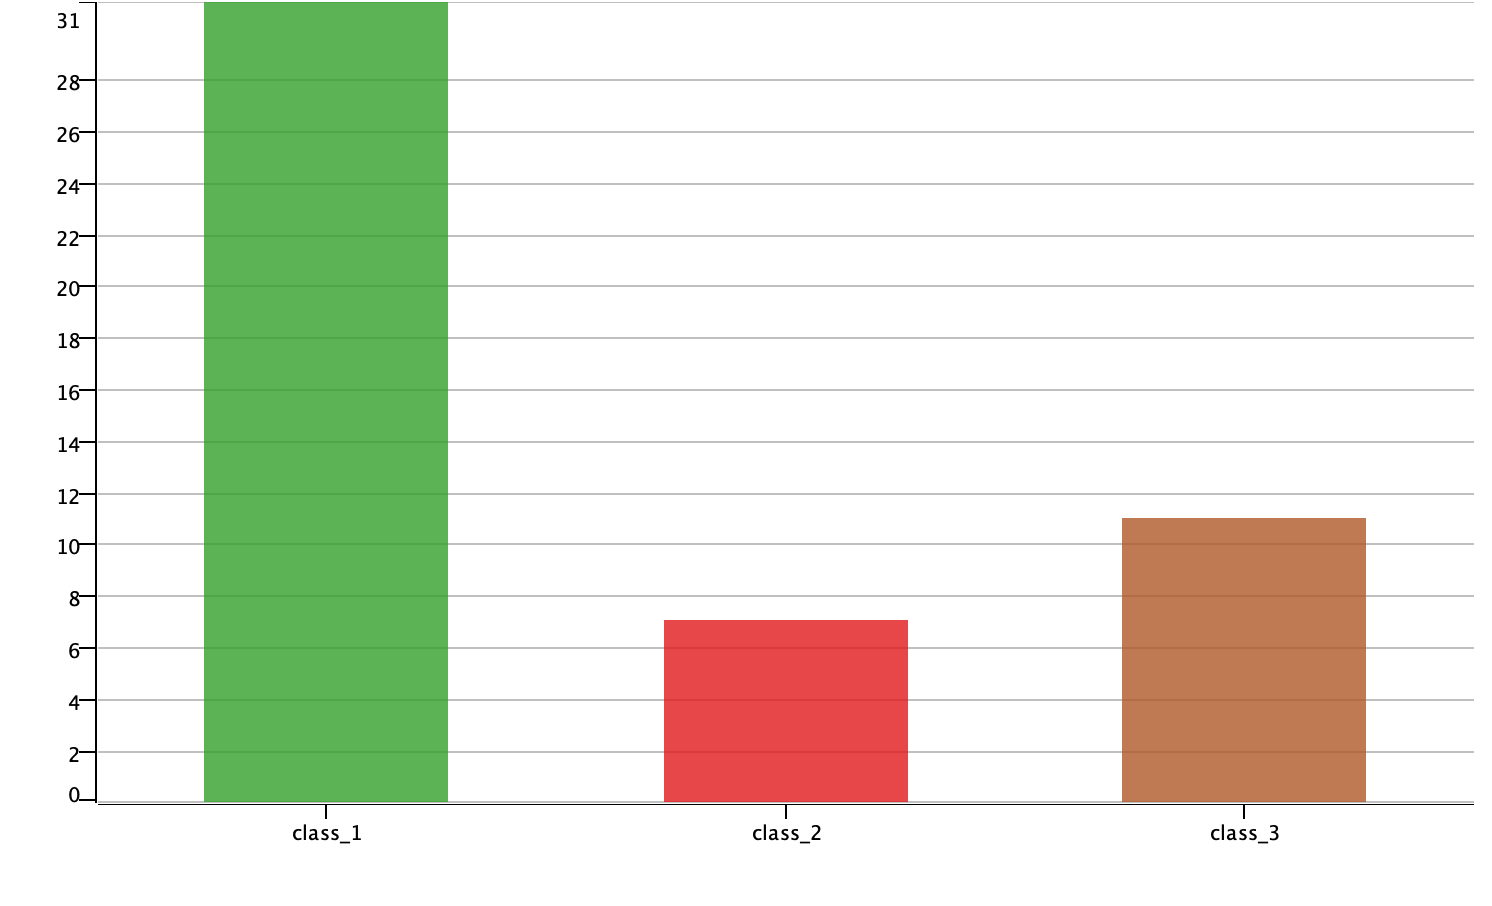
\includegraphics[width=\textwidth]{res/plot3adist}
				\caption{plot3a distribution}
				\label{fig:first}
			\end{subfigure}
			\hfill
			\begin{subfigure}{0.4\textwidth}
				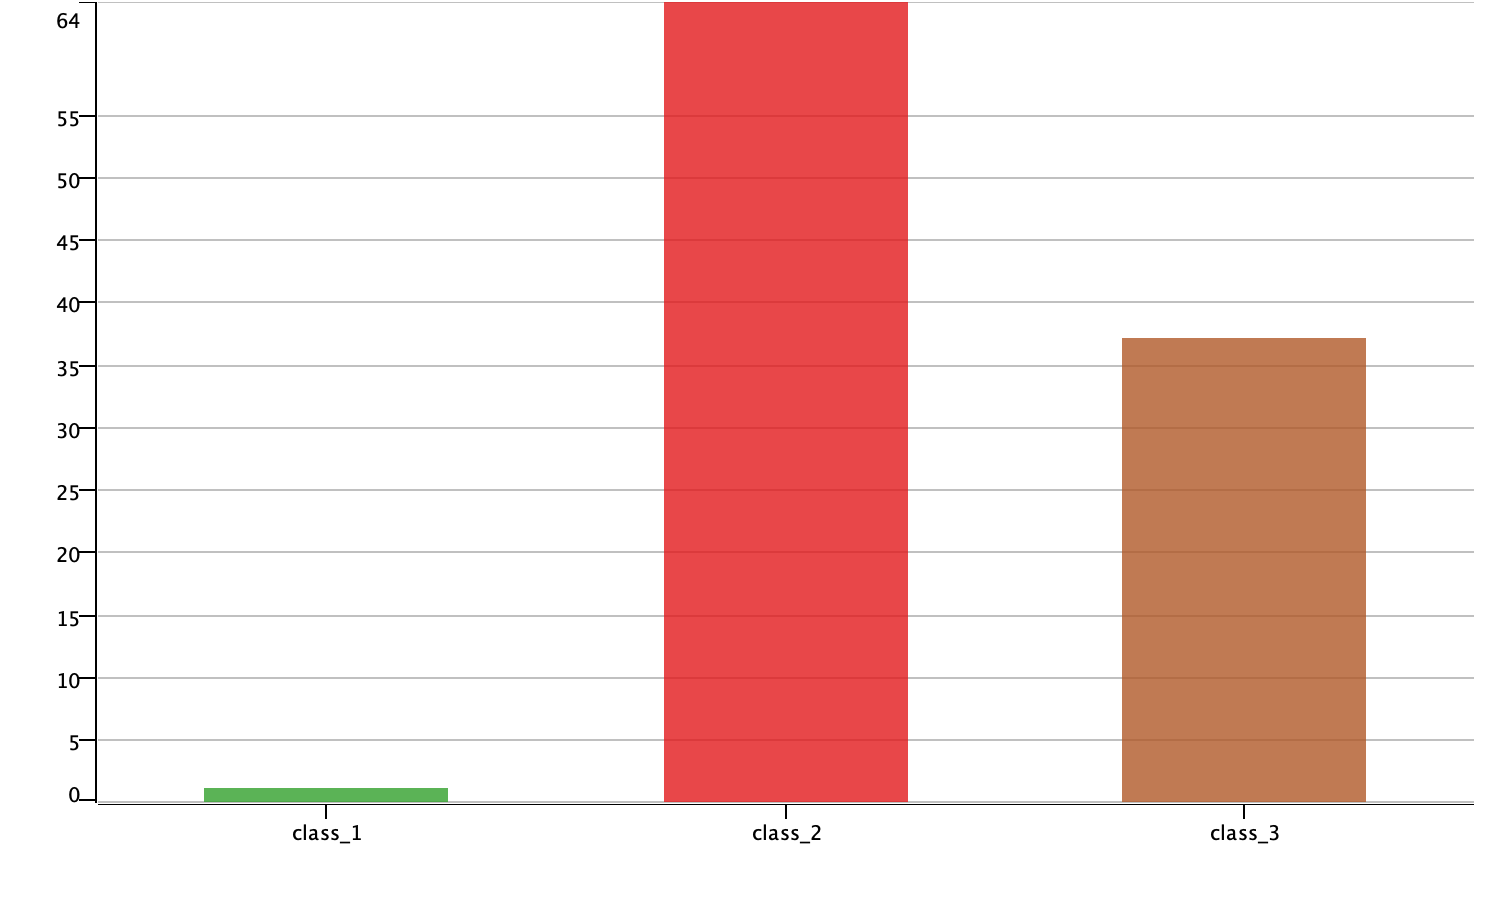
\includegraphics[width=\textwidth]{res/plot3bdist}
				\caption{plot3b distribution}
				\label{fig:second}
			\end{subfigure}
			\hfill
			\begin{subfigure}{0.4\textwidth}
				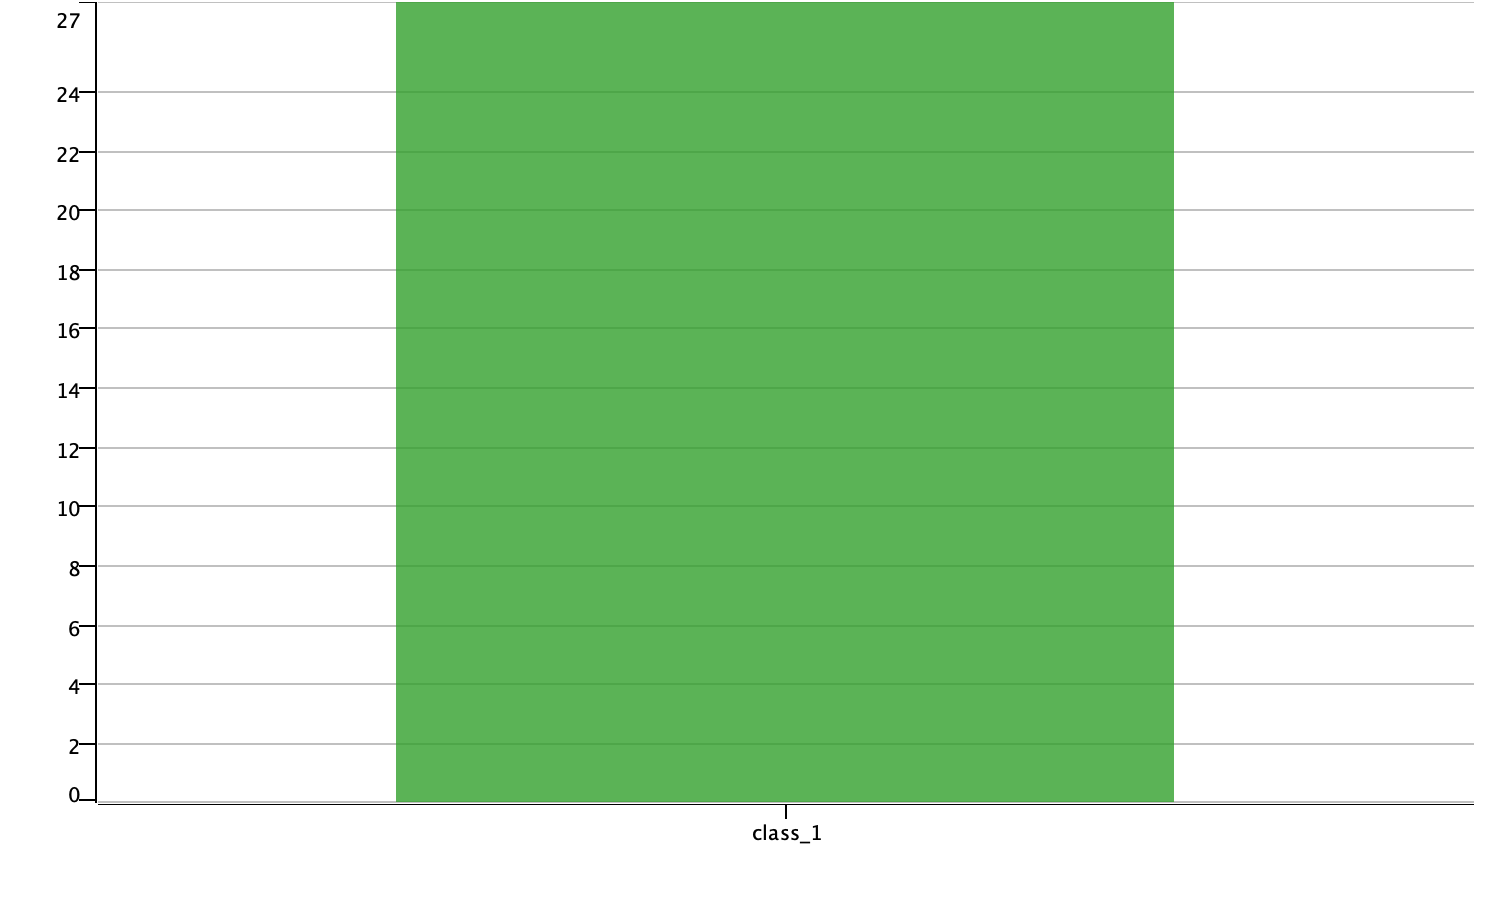
\includegraphics[width=\textwidth]{res/plot3cdist}
				\caption{plot3c distribution}
				\label{fig:third}
			\end{subfigure}
			
			\label{fig:figures}
		\end{figure}
		 This is the result of the lack of a normalization/standarization process, something that we will explain on the next task.
	
	
	%which leaves the algorithm vulnerable to distortion due to the different scales, measurement units and sizes of the variables in question. The following figure is part of the output of a simple 'Statistics' Node
	%Without Normalization
	%\begin{table}[H]
	%	\begin{tabular}{llllllllllll}
	%		Column&Min &Mean &	Median & Max  & Std. Dev.  \\
	%		Hue&0.48&0.9574&?&1.71&0.2286 \\
	%		Proline&278&746.8933&?&1,680&314.9075 \\
	%		&  &  &  & 
	%	\end{tabular}
	%\end{table}
	 
	
	
		
	
	\pagebreak
	\begin{thebibliography}{1}	
		\bibitem{free-speech-us}
		\textit{En.wikipedia.org. 2021. United States Free Speech Exceptions. [online] Available at: <https://en.wikipedia.org/wiki/United\_States\_free\_speech\_exceptions> [Accessed 10 January 2021].}
		
	\end{thebibliography}
\end{document}